\documentclass[11pt,a4paper,oneside,table,xcdraw]{article}

% CREATED BY DAVID FRISK, 2015


% BASIC SETTINGS

\usepackage{url}
\usepackage{lastpage}								% Get the number of pages
\usepackage{moreverb}								% List settings
\usepackage{textcomp}								% Fonts, symbols etc.
\usepackage{lmodern}								% Latin modern font
\usepackage{helvet}									% Enables font switching
\usepackage[T1]{fontenc}							% Output settings
\usepackage[english]{babel}							% Language settings
\usepackage[utf8]{inputenc}							% Input settings
\usepackage[table]{xcolor} 							% Table colors
\definecolor{light-gray}{gray}{0.96}			% Defining a very light gray for a table

\usepackage{amsmath}								% Mathematical expressions (American mathematical society)
\usepackage{amssymb}								% Mathematical symbols (American mathematical society)
\usepackage{graphicx}								% Figures
\usepackage{subfig}									% Enables subfigures

\usepackage{listings}								% Enables source code listings
\usepackage{xparse}								% Enables in-line code
\NewDocumentCommand{\codeword}{v}{ % Enables in-line code
	\texttt{\textcolor{blue}{#1}}
}
\usepackage{chemfig}								% Chemical structures
\usepackage[top=3cm, bottom=3cm,
			inner=3cm, outer=3cm]{geometry}			% Page margin lengths			
\usepackage{eso-pic}								% Create cover page background
\newcommand{\backgroundpic}[3]{
	\put(#1,#2){
	\parbox[b][\paperheight]{\paperwidth}{
	\centering
	\includegraphics[width=\paperwidth,height=\paperheight,keepaspectratio]{#3}}}}
\usepackage{float} 									% Enables object position enforcement using [H]
\usepackage{parskip}								% Enables vertical spaces correctly 
\usepackage{minted}
%Code highlighting and formatting
\usepackage{dirtree}
\usepackage{epigraph}
%Appendix
\usepackage[toc,page]{appendix}
\usepackage{wrapfig}
\usepackage{caption}
% OPTIONAL SETTINGS (DELETE OR COMMENT TO SUPRESS)

% Disable automatic indentation (equal to using \noindent)
\setlength{\parindent}{0cm}                         


% Caption settings (aligned left with bold name)
% \usepackage[labelfont=bf, textfont=normal,
%			justification=justified,
%			singlelinecheck=false]{caption} 		

		  	
% Activate clickable links in table of contents  	
\usepackage{hyperref}								
\hypersetup{colorlinks, citecolor=black,
   		 	filecolor=black, linkcolor=black,
    		urlcolor=black}


% Define the number of section levels to be included in the t.o.c. and numbered	(3 is default)	
\setcounter{tocdepth}{5}							
\setcounter{secnumdepth}{5}	


% Chapter title settings
\usepackage{titlesec}		
\titleformat{\chapter}
  {\Large\bfseries}{{\fontsize{35pt}{1em} {\thechapter}}}{1ex}{}[]


% Header and footer settings (Select TWOSIDE or ONESIDE layout below)
\usepackage{fancyhdr}
\pagestyle{fancy}
\fancypagestyle{plain}{}
\lhead{}
\rhead{}
\renewcommand{\chaptermark}[1]{\markboth{\thechapter.\space#1}{}}


\fancyhf{}
\fancyhead[L]{Rasmus Isager Kruuse\\Human senses and perception miniproject}
\fancyhead[R]{15/01 - 2018\\MED3}
\fancyhead[C]{}
\fancyfoot[C]{\thepage}

\usepackage[final]{pdfpages}
\usepackage{verbatim}
\usepackage{lipsum}
\usepackage{multicol}
% Enable To-do notes
\usepackage[textsize=tiny]{todonotes}   % Include the option "disable" to hide all notes
\setlength{\marginparwidth}{2.5cm} 

\usepackage{tikz}
\usetikzlibrary{mindmap,trees}
\usepackage{nameref}

% Supress warning from Texmaker about headheight
\setlength{\headheight}{30pt}		

\newcommand{\HRule}{\rule{\linewidth}{0.5mm}}

\usepackage[normalem]{ulem}
\useunder{\uline}{\ul}{}

\usepackage{tocbibind}

\usepackage{tikz}
\usepackage{pgf-pie}
\usepackage{pgfplots}
\pgfplotsset{width=12cm,compat=1.11}
\pgfplotsset{
	cycle list={red\\blue\\},
}
\usepgfplotslibrary{statistics}




\usepackage[natbibapa]{apacite} 

\begin{document}
\todo{Put in front page}
	\pagenumbering{arabic}
	\section{Introduction}
	Start with a short introduction that describes the topic and aim of the report. This should not be longer than 150 words.
	\section{What \textit{is} vection?}

	One of the problems with the term vection, is that it has been used to describe many different things by different researchers. In 2017, \cite{challenges} published a paper in which they stated four challenges that vection research currently faces. One of these is that lack of a concrete definition. They gave examples of four different definitions that was used in research. As such one should clearly define which definition that is used. In this paper i use the 1st definition, which is.
	\begin{quote}
\textit{Vection is a visual illusion of self-motion in a stationary observer}
	\end{quote}
	Following this definition vection can be described more clearly. Vection as referred to in this report is the sensation of self motion that one can get when a large part of the visual field starts moving. This often happens near large objects that such as on a ferry, on a train, or sometimes in a car. For example, if an observer is in a stationary train and the beside it starts moving. It is not uncommon to feel as if you train has started to move instead. This is vection. We are currently unsure whether vection serves a purpose in making controlling self-motion of just arises from the processing of visual data. That is, whether it has some use or is a glitch in the visual system that only occurs under very particular conditions that never happened before modernity\todo{citation maybe}. 
	\section{Theory}
\todo{Answer the following questions 3. Vection. Explain what vection is and how it differs from other types of illusory self motions one might experience. When and how can we experience vection? What determines whether it happens or not and how long the sensation lasts? }
	To understand why certain conditions can trick the human perception system into feeling self motion where there is none, we must first understand how the humans perceive motion, and why this causes no problems under normal conditions. This section covers the theory of human motion perception. 
\subsection{Motion perception}
	As with many of the processes that goes on in the brain, exactly how it understands motion is not understood. It is known that multiple process are involved in perceiving motion\todo{Find citation}. At least two process are involved. 
\begin{figure}
	\centering
	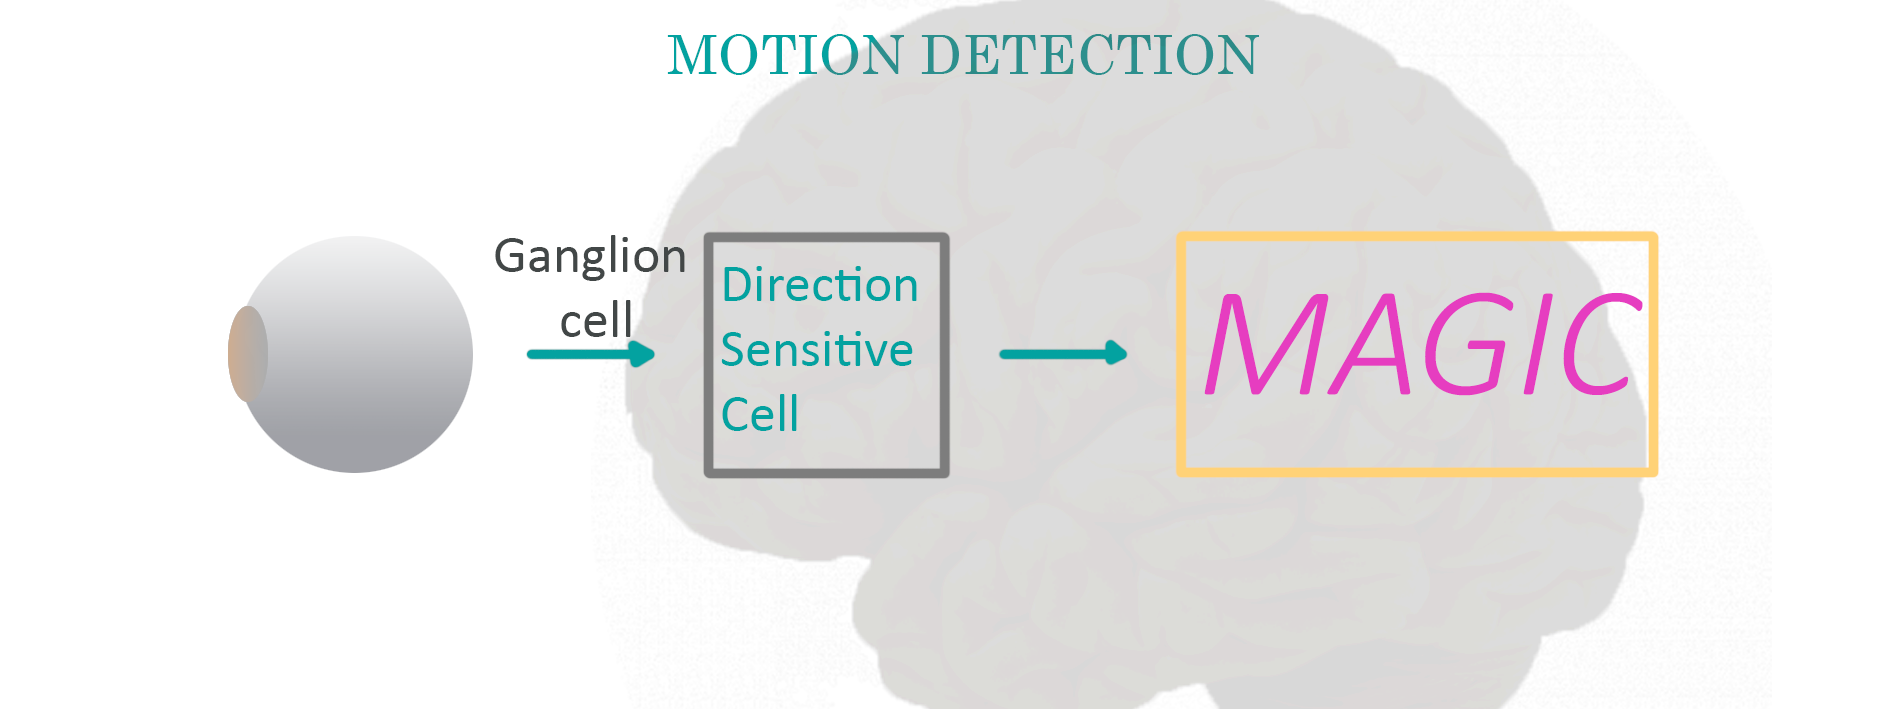
\includegraphics[width=0.9\linewidth]{figure/process.png}
	\caption{WIP model explaining the order of the next sections}
	\label{fig:process}
\end{figure}
	\subsection{Direction sensitive cells}
	\subsection{Direction sensitive neurons}
	
	As a guideline, someone reading your report should be able to answer the questions/tasks stated for the topic after having read it. The more you understand your topic and can explain it in your own words, the greater the likelihood is that you succeed.\\\\
	Report the theory relevant to your topic and the questions you are to answer. The available course literature (e.g. Yantis \& Abrams, 2017; Wolfe et al., 2015; Snowden, Thompson, \& Troscianko, 2006) are good starting points, but to get more specific information and achieve a higher grade you should also search for and read review articles (e.g. Elliot 2015; Elliott, Vale, Whitaker \& Buckley, 2009), and other relevant information. Use the suggested readings or references listed in your course book as a starting point and search for related articles and articles that have been citing the earlier ones.\\\\
	If you have any questions regarding your report, please contact your teacher in reasonable time before hand in. The weekend of delivery is NOT reasonable.

	\section{Discussion}
	After you have reported the theory and clarified or answered the questions stated in
	the topic you should devote about one page to put this into context. Try to think of
	what it means for everyday life and our usage of digital media. Find examples! What
	should one take into consideration when designing multimedia applications? How can
	you use the knowledge in your semester project?
	Similarly, if you have reported own experiments you also need to put this in
	perspective: Could you have used other approaches, references or theories? Did
	anything go wrong (weaknesses)? What was good (strength)? Create relevant
	subheadings that depict the topics you have extrapolated. 
\bibliographystyle{apacite}
\bibliography{include/backmatter/bibliography}
	
\end{document}